% Created 2012-10-30 mar 11:32
\documentclass[bigger]{beamer}
\usetheme{Madrid}\usecolortheme{default} \institute[FaI - UNCo]{Facultad de Inform\'atica - Universidad Nacional del Comahue}
\usepackage[utf8]{inputenc}
\usepackage[T1]{fontenc}
\usepackage{graphicx}
\usepackage{longtable}
\usepackage{float}
\usepackage{wrapfig}
\usepackage{soul}
\usepackage{amssymb}
\usepackage{hyperref}
\usepackage[spanish]{babel} \usepackage{amssymb} \usepackage{amsthm} \usepackage{float}
\usepackage[colorlinks=true,linkcolor=black,citecolor=black,urlcolor= blue,breaklinks=true,naturalnames=true]{hyperref}
\usepackage{url}
\AtBeginSection[]{\begin{frame}<beamer>\frametitle{Sección Actual}\tableofcontents[currentsection]\end{frame}}

\title{Planificación Continua mediante PDDL}
\author{Germán Braun}
\date{30 de Octubre de 2012}

\begin{document}

\maketitle










\begin{frame}<beamer>\frametitle{Agenda}\tableofcontents \end{frame}

\section{Motivación}
\label{sec-1}
\begin{frame}[<+->]
\frametitle{Motivación}
\label{sec-1.1}
\begin{itemize}

\item \textbf{Planificación Continua}\\
\label{sec-1.1.1}%
\item \textbf{Lenguaje de Definición de Dominios de Planificación (PDDL)}\\
\label{sec-1.1.2}%
\end{itemize} % ends low level
%% Asimo
\label{sec-1.1.3}

\begin{center} 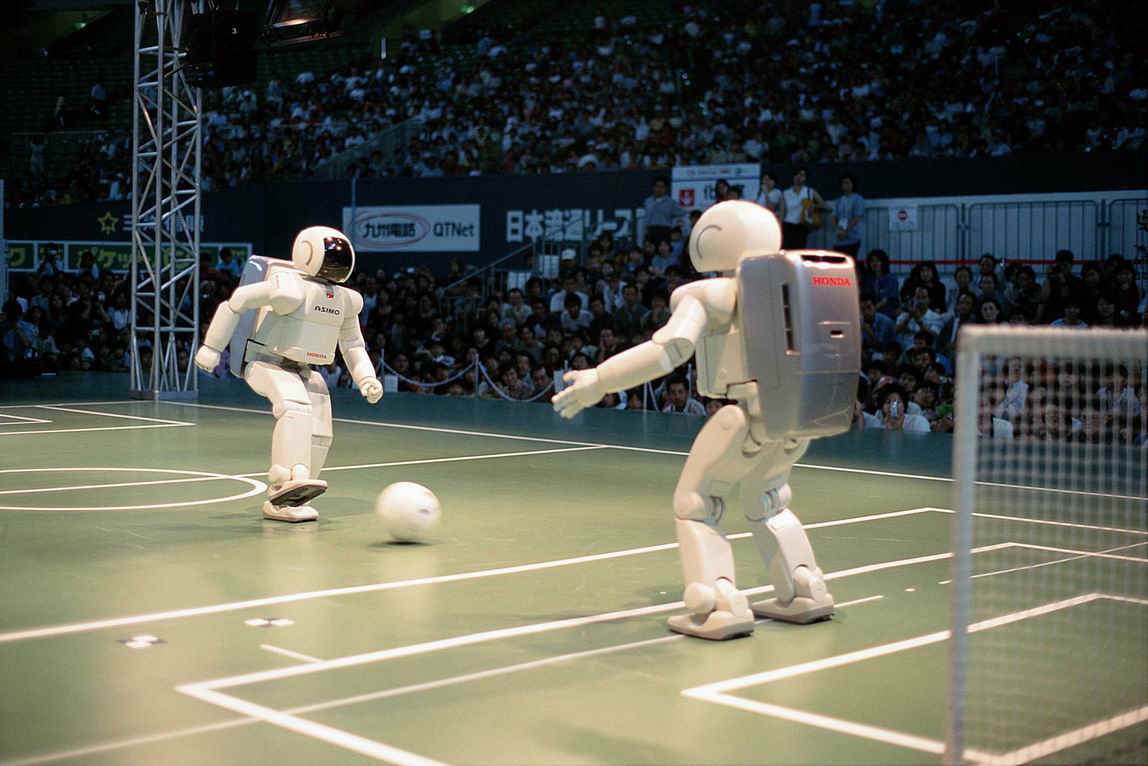
\includegraphics[width=7.5cm,height=4.5cm]{asimo.png} \end{center}
\href{http://asimo.honda.com/}{http://asimo.honda.com/}
\end{frame}
\begin{frame}
\frametitle{Planificación (1)}
\label{sec-1.2}

\begin{center} 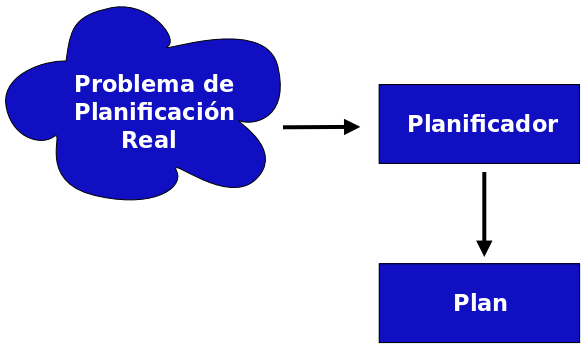
\includegraphics[width=10cm,height=6cm]{planificacion1.png} \end{center}
\end{frame}
\begin{frame}
\frametitle{Planificación (2) - Ejemplo}
\label{sec-1.3}

\begin{center} 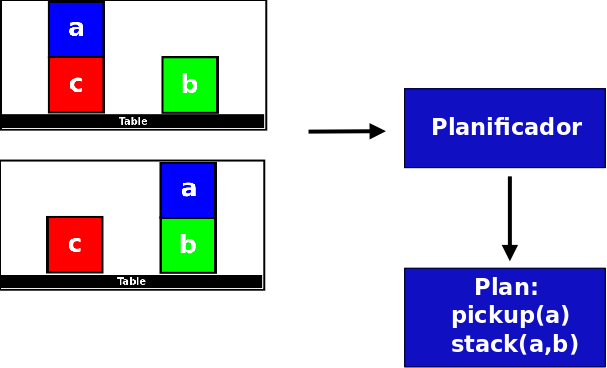
\includegraphics[width=10cm,height=6cm]{planificacion1-1.png} \end{center}
\end{frame}
\begin{frame}
\frametitle{Planificación (3)}
\label{sec-1.4}

\begin{center} 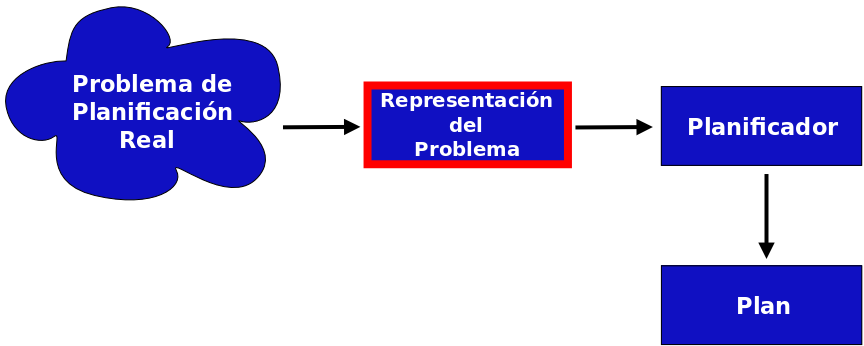
\includegraphics[width=11.5cm,height=5cm]{planificacion2.png} \end{center}
\end{frame}
\begin{frame}
\frametitle{Planificación (4) - Ejemplo}
\label{sec-1.5}

\begin{center} 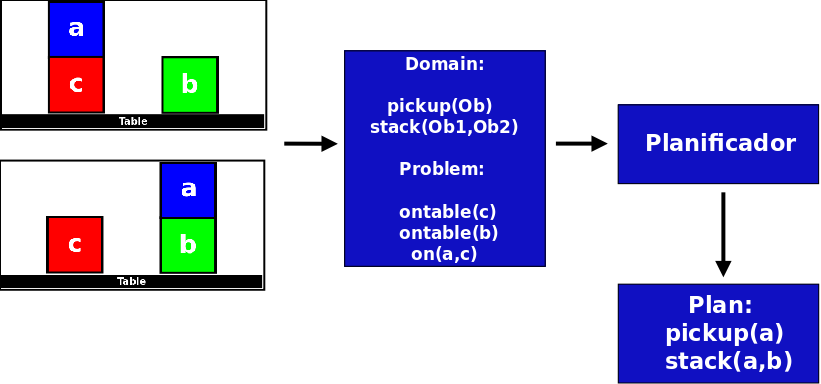
\includegraphics[width=11cm,height=5cm]{planificacion2-1.png} \end{center}
\end{frame}
\begin{frame}
\frametitle{Planificación (5)}
\label{sec-1.6}

\begin{center} 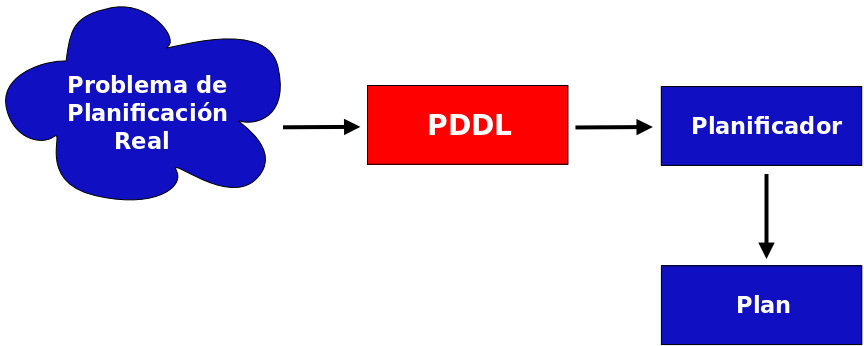
\includegraphics[width=11.5cm,height=5cm]{pddl.png} \end{center}
\end{frame}
\begin{frame}[<+->]
\frametitle{Planificación (6) - PDDL}
\label{sec-1.7}
\begin{itemize}

\item \textbf{Lenguaje estándar}
\label{sec-1.7.1}%
\begin{itemize}

\item \emph{Ampliamente aceptado por la comunidad IA}\\
\label{sec-1.7.1.1}%
\end{itemize} % ends low level

\item \textbf{Requerimientos}
\label{sec-1.7.2}%
\begin{itemize}

\item \emph{strips (``núcleo''), igualdad, efectos condicionales, precondiciones disyuntivas, precondiciones universales\ldots{}}\\
\label{sec-1.7.2.1}%
\end{itemize} % ends low level

\item \textbf{Action-centered}
\label{sec-1.7.3}%
\begin{itemize}

\item \emph{Listas de precondiciones y efectos}\\
\label{sec-1.7.3.1}%
\end{itemize} % ends low level

\item \textbf{Dominio}
\label{sec-1.7.4}%
\begin{itemize}

\item \emph{Acciones parametrizadas, Predicados, Constantes\ldots{}}\\
\label{sec-1.7.4.1}%
\end{itemize} % ends low level

\item \textbf{Problema}
\label{sec-1.7.5}%
\begin{itemize}

\item \emph{Objetos, metas y condiciones iniciales\ldots{}}\\
\label{sec-1.7.5.1}%
\end{itemize} % ends low level
\end{itemize} % ends low level
\end{frame}
\begin{frame}[fragile]
\frametitle{Planificación (7) - Dominio PDDL}
\label{sec-1.8}
\begin{block}{Ejemplo: \emph{Dominio PDDL}}
\label{sec-1.8.1}

 \begin{verbatim}
(define (domain bkw)
(:requirements :strips)
(:predicates (clear ?x) (ontable ?x) (armempty)
             (holding ?x) (on ?x ?y))

(:action stack
  :parameters  (?ob ?underob)
  :precondition (and  (clear ?underob) (holding ?ob))
  :effect (and (clear ?ob) (on ?ob ?underob) (armempty)
               (not(clear ?underob)) 
               (not(holding ?ob)))))
 \end{verbatim}
\end{block}
\end{frame}
\begin{frame}[fragile]
\frametitle{Planificación (8) - Problema PDDL}
\label{sec-1.9}
\begin{block}{Ejemplo: \emph{Problema PDDL}}
\label{sec-1.9.1}

 \begin{verbatim}
(define (problem pb1)
   (:domain bkw)
   (:objects a b)
   (:goal (on a b))
   (:init (ontable c) (ontable b) 
          (on a c) (clear a) (clear b) (armempty))
)
 \end{verbatim}
\end{block}
\end{frame}
\begin{frame}
\frametitle{Planificación (9)}
\label{sec-1.10}

\begin{center} 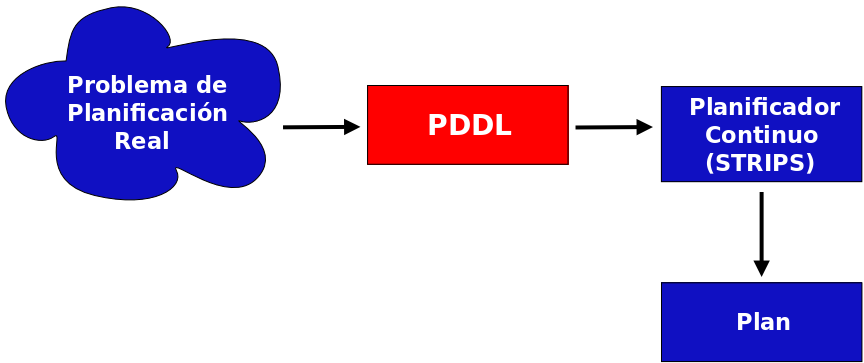
\includegraphics[width=11.5cm,height=5cm]{planificacion-final.png} \end{center}
\end{frame}
\begin{frame}
\frametitle{Motivación Principal}
\label{sec-1.11}
\begin{block}{Motivación}
\label{sec-1.11.1}


Dotar al Planificador Continuo\footnote{Tesis Mario Moya: ``Control de Agentes Basado en Planificación Continua''. } de un módulo traductor del lenguaje
PDDL, permitiendo que el sistema de creencias de un agente soporte
percepciones y acciones especificadas en este lenguaje.
\end{block}
\end{frame}
\begin{frame}
\frametitle{Motivación Principal - Aplicaciones}
\label{sec-1.12}
\begin{columns}
\begin{column}{0.4\textwidth}
%% SAP speaks PDDL
\label{sec-1.12.1}

\begin{center} 
\includegraphics[width=4.5cm,height=3cm]{sap.png}\\\caption{\textbf{SAP speaks PDDL}}\end{center}
    
\end{column}
\begin{column}{0.4\textwidth}
%% Planning aplicado a e-learning
\label{sec-1.12.2}

\begin{center} 
\includegraphics[width=4cm,height=3cm]{moodle.png}\\\caption{\textbf{Planning aplicado a e-learning}}\end{center}
\end{column}
\end{columns}
\end{frame}
\section{Objetivos}
\label{sec-2}
\begin{frame}
\frametitle{Objetivos (1)}
\label{sec-2.1}
\begin{block}{Objetivo}
\label{sec-2.1.1}

Implementar un módulo capaz de procesar problemas de \emph{pla\-ni\-fi\-ca\-ción}
en un subconjunto de \emph{PDDL} y generar una especificación equivalente
en el lenguaje \emph{STRIPS} del \emph{Planificador Continuo}.
\end{block}
\end{frame}
\begin{frame}
\frametitle{Objetivos (2)}
\label{sec-2.2}

\begin{center} 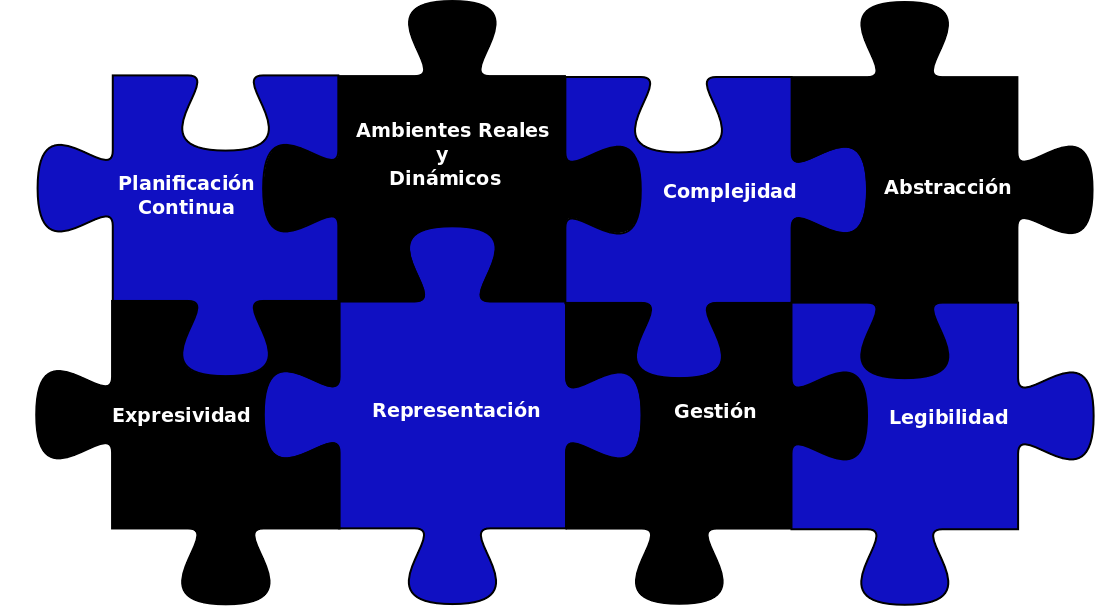
\includegraphics[width=11cm,height=7cm]{puzzle.png} \end{center}
\end{frame}
\section{Traductor en Ciao Prolog}
\label{sec-3}
\begin{frame}[<+->]
\frametitle{Traductor en Ciao Prolog}
\label{sec-3.1}
\begin{itemize}

\item \textbf{Lenguaje Fuente}
\label{sec-3.1.1}%
\begin{itemize}

\item \emph{Subconjunto de PDDL}\\
\label{sec-3.1.1.1}%
\item \emph{Formalismos como variantes de PDDL}
\label{sec-3.1.1.2}%
\begin{itemize}

\item División por requerimientos.\\
\label{sec-3.1.1.2.1}%
\item \textbf{:strips} es incluido por defecto.\\
\label{sec-3.1.1.2.2}%
\end{itemize} % ends low level
\end{itemize} % ends low level
\end{itemize} % ends low level
\end{frame}
\begin{frame}[fragile,<+->]
\frametitle{Lenguaje Fuente - STRIPS}
\label{sec-3.2}
\begin{itemize}

\item :strips -> PDDL$_{STRIPS}$\\
\label{sec-3.2.1}%
\end{itemize} % ends low level
\begin{block}{Ejemplo: \emph{PDDL$_{\mathrm{STRIPS}}$}}
\label{sec-3.2.2}

 \begin{verbatim}
(:action stack
  :parameters  (?ob ?underob)
  :precondition (and  (clear ?underob) (holding ?ob))
  :effect (and (clear ?ob) (on ?ob ?underob) (armempty)
               (not (clear ?underob)) 
               (not (holding ?ob)))))
 \end{verbatim}
\end{block}
\end{frame}
\begin{frame}[fragile,<+->]
\frametitle{Lenguaje Fuente - Igualdad}
\label{sec-3.3}
\begin{itemize}

\item :equality -> PDDL$_{L}$\\
\label{sec-3.3.1}%
\end{itemize} % ends low level
\begin{block}{Ejemplo: \emph{PDDL$_{L}$}}
\label{sec-3.3.2}

 \begin{verbatim}
 (:action stack
   :parameters (?X ?Y)
   :precondition (and (clear table) (= ?Y table)) 
   :effect (and (on ?X table) (not (clear table))))

 (:action stack1
   :parameters (?X ?Y)
   :precondition (and (clear ?Y) (not (= ?Y table))) 
   :effect (and (on ?X ?Y) (not (clear ?Y))))                 
 \end{verbatim}
\end{block}
\end{frame}
\begin{frame}[fragile,<+->]
\frametitle{Lenguaje Fuente - Efectos Condicionales}
\label{sec-3.4}
\begin{itemize}

\item :conditional-effect -> PDDL$_{\emph{C}}$\\
\label{sec-3.4.1}%
\end{itemize} % ends low level
\begin{block}{Ejemplo: \emph{PDDL$_{C}$}}
\label{sec-3.4.2}

 \begin{verbatim}
(:action stack
   :parameters (?X ?Y ?Z)
   :precondition (and (clear ?X) (clear ?Z) (on ?X ?Y))
   :effects (and (on ?X ?Z) (clear ?Y) (not (on ?X ?Y)) 
                 (when (not (= table ?Z)) 
                       (not (clear ?Z)))))
 \end{verbatim}
\end{block}
\end{frame}
\begin{frame}[fragile,<+->]
\frametitle{Lenguaje Fuente - Precondiciones Disyuntivas}
\label{sec-3.5}
\begin{itemize}

\item :disjuntive-preconditions -> PDDL$_{D}$\\
\label{sec-3.5.1}%
\end{itemize} % ends low level
\begin{block}{Ejemplo: \emph{PDDL$_{D}$}}
\label{sec-3.5.2}

 \begin{verbatim}
(:action stack
   :parameters (?X ?Y ?Z)
   :precondition (and (or (istable ?Z) (clear ?Z))
                      (clear ?X) (on ?X ?Y))
   :effect (and (on ?X ?Z) (clear ?Y)
                (not (clear ?Y)) 
                (not (on ?X ?Y))))
 \end{verbatim}
\end{block}
\end{frame}
\begin{frame}[fragile,<+->]
\frametitle{Lenguaje Fuente - Precondiciones Universales}
\label{sec-3.6}
\begin{itemize}

\item :universal-preconditions -> PDDL$_{\emph{u}}$\\
\label{sec-3.6.1}%
\end{itemize} % ends low level
\begin{block}{Ejemplo: \emph{PDDL$_{u}$}}
\label{sec-3.6.2}

 \begin{verbatim}
(:action stack
  :parameters  (?ob ?underob)
  :precondition (and (forall (?block) (ontable ?block))
                     (clear ?underob) (holding ?ob))
  :effect (and (clear ?ob) (on ?ob ?underob) (armempty)
               (not (clear ?underob)) 
               (not (holding ?ob))))
 \end{verbatim}



    

    




        
\end{block}
\end{frame}
\begin{frame}[<+->]
\frametitle{Lenguaje Destino}
\label{sec-3.7}
\begin{itemize}

\item \textbf{Lenguaje Destino}
\label{sec-3.7.1}%
\begin{itemize}

\item \emph{Representación Genérica (Prolog-like)}
\label{sec-3.7.1.1}%
\begin{itemize}

\item \emph{Independiente del Planificador destino}\\
\label{sec-3.7.1.1.1}%
\item \emph{Permite adaptar el traductor a otros Planificadores basados en STRIPS}\\
\label{sec-3.7.1.1.2}%
\item \textbf{Nuestra Implementación}: \emph{STRIPS-like} -> \emph{Es el lenguaje del Planificador Continuo y se obtiene a partir de la representación genérica anterior}\\
\label{sec-3.7.1.1.3}%
\end{itemize} % ends low level
\end{itemize} % ends low level
\end{itemize} % ends low level
\end{frame}
\begin{frame}[fragile]
\frametitle{Representación Genérica - Dominio}
\label{sec-3.8}
\begin{block}{Definición: \emph{Dominio}}
\label{sec-3.8.1}

 \begin{verbatim}
preconditions(action_name_i(parameters), 
          [predicate_j(parameters_k),...]).
   
achieves(action_name_i(parameters),
          [predicate_j(parameters_k),...]).

deletes(action_name_i(parameters),
          [predicate_j(parameters_k),...]).
 \end{verbatim}
\end{block}
\end{frame}
\begin{frame}[fragile]
\frametitle{Representación Genérica - Problema}
\label{sec-3.9}
\begin{block}{Definición: \emph{Problema}}
\label{sec-3.9.1}

 \begin{verbatim}
(domain(domain_name),
  objects(obj_1,obj_2,..,obj_N),
  goal(fact_g),
  init(fact_1,fact_2,..,fact_N)).
 \end{verbatim}
\end{block}
\end{frame}
\section{Demostración}
\label{sec-4}
\begin{frame}
\frametitle{DEMO}
\label{sec-4.1}
\begin{columns}
\begin{column}{0.4\textwidth}
%% Estado Inicial
\label{sec-4.1.1}

    \begin{center}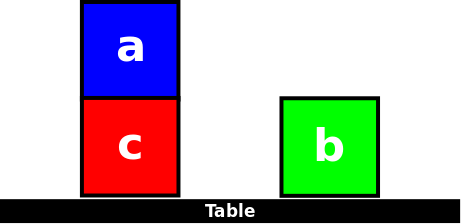
\includegraphics[width=5cm,height=2.5cm]{bkwInicial.png}\\\caption{Estado Inicial}\end{center}
    
\end{column}
\begin{column}{0.4\textwidth}
%% Estado Final
\label{sec-4.1.2}

    \begin{center}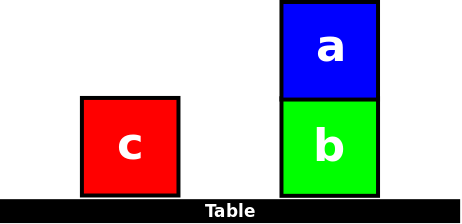
\includegraphics[width=5cm,height=2.5cm]{bkwFinal.png}\\\caption{Estado Final}\end{center}
\end{column}
\end{columns}
\end{frame}
\section{Traducción de Requerimientos}
\label{sec-5}
\begin{frame}[<+->]
\frametitle{Traducción ¿Cómo es?}
\label{sec-5.1}
\begin{itemize}

\item \textbf{Conceptos}
\label{sec-5.1.1}%
\begin{itemize}

\item \emph{Esquemas de Compilación}\\
\label{sec-5.1.1.1}%
\item \emph{Compilabilidad}\\
\label{sec-5.1.1.2}%
\end{itemize} % ends low level
\end{itemize} % ends low level
\end{frame}
\begin{frame}[<+->]
\frametitle{Traducción - Esquemas de Compilación}
\label{sec-5.2}
\begin{itemize}

\item Básicamente, un \textbf{esquema de compilación} es un mapeo entre dos formalismos de planificación X e Y.\\
\label{sec-5.2.1}%
\end{itemize} % ends low level
\begin{block}{Definición: \emph{Esquemas de Compilación}}
\label{sec-5.2.2}

$F(\Pi) = \left\langle f_{\xi}(\Xi),I \cup f_{i}(\Xi),G \cup
f_{g}(\Xi) \right\rangle$, donde $\Xi$ es un dominio, $I$ es el estado
inicial y $G$ es un conjunto de metas.
\end{block}
\begin{block}{Condición Importante}
\label{sec-5.2.3}

Existe un plan para $\Pi$, si y solo si, existe un plan para $F(\Pi)$,
donde $\Pi$ es la definición del dominio en el formalismo X y $F(\Pi)$
es la definición del dominio en el formalismo Y.
\end{block}
\end{frame}
\begin{frame}[<+->]
\frametitle{Traducción - Compilabilidad (1)}
\label{sec-5.3}
\begin{itemize}

\item Los esquemas de compilación permiten definir una relación entre formalismos, llamada \emph{Compilabilidad (Compilability)}.\\
\label{sec-5.3.1}%
\end{itemize} % ends low level
\begin{block}{Definición: \emph{Compilabilidad}}
\label{sec-5.3.2}

        Un formalismo de planificaci\'on $X$ es {\bf compilable} al formalismo 
        $Y$, expresado como $X \preccurlyeq^{x} Y$, si y s\'olo si,
        existe un esquema de compilaci\'on de $X$ a $Y$.
\end{block}
\end{frame}
\begin{frame}[<+->]
\frametitle{Compilabilidad (2)}
\label{sec-5.4}
\begin{itemize}

\item Si \textbf{X \preccurlyeq$^{1}$ Y}, entonces el tamaño del plan es preservado exactamente.\\
\label{sec-5.4.1}%
\item Si \textbf{X \preccurlyeq$^{c}$ Y}, entonces el tamaño del plan es preservado linealmente (en $||\Delta||$), donde $||\Delta||$ es el tamaño del plan obtenido en X.\\
\label{sec-5.4.2}%
\item Si \textbf{X \preccurlyeq$^{p}$ Y}, entonces el tamaño del plan es preservado polinomialmente (en $||\Delta||$ y $||\Pi||$), donde $||\Pi||$ es el número de acciones en X.\\
\label{sec-5.4.3}%
\item Si \textbf{X \preccurlyeq$^{x}$$_{p}$ Y}, entonces la compilación es en tiempo polinomial y el tamaño del plan es preservado polinomialmente (en $||\Delta||$ y $||\Pi||$).\\
\label{sec-5.4.4}%
\end{itemize} % ends low level
\end{frame}
\begin{frame}[<+->]
\frametitle{Compilabilidad (3)}
\label{sec-5.5}
\begin{itemize}

\item Entonces, considerando el lenguaje fuente y destino de nuestra implementación, definimos las siguientes relaciones:
\label{sec-5.5.1}%
\begin{itemize}

\item \textbf{PDDL$_{\mathrm{STRIPS}}$} \preccurlyeq$^{1}$ \textbf{STRIPS}\\
\label{sec-5.5.1.1}%
\item \textbf{PDDL$_{L}$} \preccurlyeq$^{1}$$_{p}$ \textbf{STRIPS}\\
\label{sec-5.5.1.2}%
\item \textbf{PDDL$_{C}$} \preccurlyeq$^{x}$$_{p}$ \textbf{STRIPS}\\
\label{sec-5.5.1.3}%
\item \textbf{PDDL$_{D}$} \preccurlyeq$^{1}$$_{p}$ \textbf{STRIPS}\\
\label{sec-5.5.1.4}%
\item \textbf{PDDL$_{u}$} \preccurlyeq$^{1}$$_{p}$ \textbf{STRIPS}\\
\label{sec-5.5.1.5}%
\end{itemize} % ends low level
\end{itemize} % ends low level
\end{frame}
\begin{frame}[fragile]
\frametitle{Compilabilidad - Ejemplo (1)}
\label{sec-5.6}
\begin{itemize}

\item \textbf{PDDL$_{u}$} \preccurlyeq$^{1}$$_{p}$ \textbf{STRIPS}\\
\label{sec-5.6.1}%
\end{itemize} % ends low level
\begin{block}{Ejemplo: \emph{Problema}}
\label{sec-5.6.2}

 \begin{verbatim}
(define (problem pb1)
   (:domain bkwup)
   (:objects a b c)
   (:goal (on a b))
   (:init (ontable c) (ontable b) (ontable a) 
          (on a c) (clear a) (clear b) (armempty))
)
 \end{verbatim}
\end{block}
\end{frame}
\begin{frame}[fragile]
\frametitle{Compilabilidad - Ejemplo (2)}
\label{sec-5.7}
\begin{block}{Ejemplo: \emph{Dominio}}
\label{sec-5.7.1}

 \begin{verbatim}
(:action stack
  :parameters  (?ob ?underob)
  :precondition (and (forall (?block) (ontable ?block))
                     (clear ?underob) (holding ?ob))
  :effect (and (clear ?ob) (on ?ob ?underob) (armempty)
               (not (clear ?underob)) 
               (not (holding ?ob))))
 \end{verbatim}
\end{block}
\end{frame}
\begin{frame}[fragile]
\frametitle{Compilabilidad - Ejemplo (3)}
\label{sec-5.8}
\begin{block}{Ejemplo: \emph{STRIPS}}
\label{sec-5.8.1}

 \begin{verbatim}
% stack(X,Y)
preconditions(stack(X,Y),[ontable(a),ontable(b),
                          ontable(c),
                          clear(Y),holding(X)]).
deletes(stack(X,Y),clear(Y)).
deletes(stack(X,Y),holding(X)).
achieves(stack(X,Y),clear(X)).
achieves(stack(X,Y),on(X,Y)).
achieves(stack(X,Y),armempty).
 \end{verbatim}
\end{block}
\end{frame}
\begin{frame}
\frametitle{Arquitectura Modular}
\label{sec-5.9}

\begin{center} 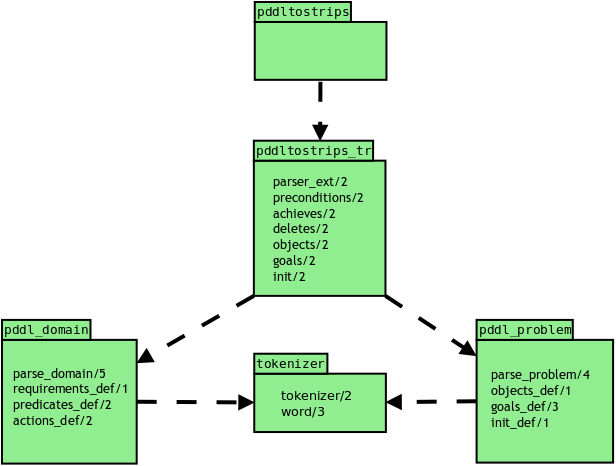
\includegraphics[width=9.5cm,height=7cm]{UMLParser.png} \end{center} 
\end{frame}
\section{Conclusiones}
\label{sec-6}
\begin{frame}
\frametitle{Resultados (1)}
\label{sec-6.1}
\begin{block}{Teorema}
\label{sec-6.1.1}

#$STRIPS_{\emph{u}} \preccurlyeq^{1}_{p} STRIPS$
\end{block}
\begin{block}<2->{Corolario}
\label{sec-6.1.2}

#$PDDL_{\emph{u}} \preccurlyeq^{1}_{p} STRIPS$
\end{block}
\end{frame}
\begin{frame}[<+->]
\frametitle{Resultados (2)}
\label{sec-6.2}
\begin{itemize}

\item \textbf{PDDL$_{\mathrm{STRIPS}}$}
\label{sec-6.2.1}%
\begin{itemize}

\item Requerimiento :strips\\
\label{sec-6.2.1.1}%
\end{itemize} % ends low level

\item \textbf{PDDL$_{L}$}
\label{sec-6.2.2}%
\begin{itemize}

\item Requerimiento :equality\\
\label{sec-6.2.2.1}%
\end{itemize} % ends low level

\item \textbf{PDDL$_{C}$}
\label{sec-6.2.3}%
\begin{itemize}

\item Requerimiento: conditional-effect\\
\label{sec-6.2.3.1}%
\end{itemize} % ends low level

\item \textbf{PDDL$_{D}$}
\label{sec-6.2.4}%
\begin{itemize}

\item Requerimiento: disjuntive-preconditions\\
\label{sec-6.2.4.1}%
\end{itemize} % ends low level
\end{itemize} % ends low level
\end{frame}
\begin{frame}
\frametitle{Adaptación a otros Planificadores}
\label{sec-6.3}

\begin{center}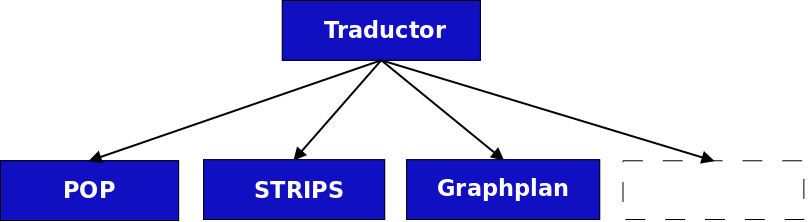
\includegraphics[width=11.5cm,height=3.5cm]{adaptacion.png}\end{center}
\end{frame}
\begin{frame}
\frametitle{Integración con el Framework de Planificación Continua}
\label{sec-6.4}

\begin{center}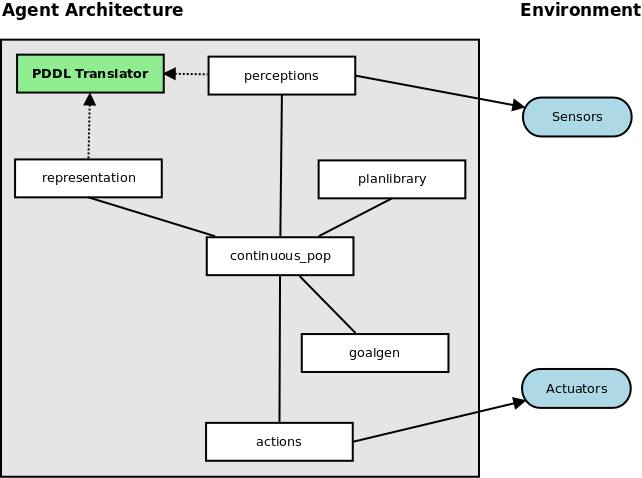
\includegraphics[width=7.5cm,height=6.5cm]{arqframework.png}\end{center}
\end{frame}
\begin{frame}
\frametitle{Expansión Sintáctica para Ciao Prolog}
\label{sec-6.5}

\begin{center}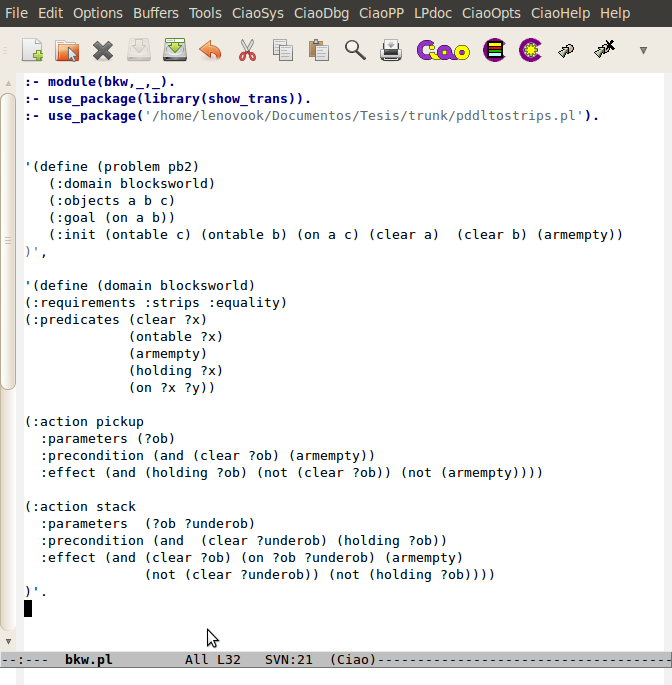
\includegraphics[width=7.5cm,height=7.5cm]{demoPddlCiao.png}\end{center}
\end{frame}
\begin{frame}[<+->]
\frametitle{Trabajo Futuro}
\label{sec-6.6}
\begin{itemize}

\item \textbf{Ampliar el Lenguaje Fuente del Traductor}
\label{sec-6.6.1}%
\begin{itemize}

\item \emph{Definir esquemas de compilación asociados.}\\
\label{sec-6.6.1.1}%
\end{itemize} % ends low level

\item \textbf{Análisis exhaustivo de la complejidad del Traductor}
\label{sec-6.6.2}%
\begin{itemize}

\item \emph{Disminuir el impacto de la traducción en la planificación.}\\
\label{sec-6.6.2.1}%
\end{itemize} % ends low level

\item \textbf{Interface para el Framework de Planificación Continua}
\label{sec-6.6.3}%
\begin{itemize}

\item \emph{Pruebas sobre dominios reales.}\\
\label{sec-6.6.3.1}%
\item \emph{Traducción de percepciones en tiempo real.}\\
\label{sec-6.6.3.2}%
\end{itemize} % ends low level

\item \textbf{Aplicar conceptos de Compiladores e Intérpretes}
\label{sec-6.6.4}%
\begin{itemize}

\item \emph{Manipulación y Recuperación de Errores.}\\
\label{sec-6.6.4.1}%
\end{itemize} % ends low level

\item \textbf{Combinar el Traductor con otros Planificadores}
\label{sec-6.6.5}%
\begin{itemize}

\item \emph{Realizar comparaciones de performance.}\\
\label{sec-6.6.5.1}%
\end{itemize} % ends low level
\end{itemize} % ends low level
\end{frame}
\begin{frame}
\frametitle{Fin}
\label{sec-6.7}

%\vspace{0.5cm}
\hspace{4.5cm}
{\bf ¿Preguntas?}
\end{frame}
\begin{frame}
\frametitle{¡Gracias!}
\label{sec-6.8}

\href{http://code.google.com/p/my-pddl-to-strips-tesis/}{http://code.google.com/p/my-pddl-to-strips-tesis/}
\begin{center}
\includegraphics[width=6cm,height=6cm]{qrplanet.png}\end{center}
\end{frame}
\begin{frame}[<+->]
\frametitle{Anexo (1) - Implementaciones Existentes}
\label{sec-6.9}
\begin{itemize}

\item \textbf{Analizador en SWI-Prolog}
\label{sec-6.9.1}%
\begin{itemize}

\item \emph{Otra implementación Prolog}\\
\label{sec-6.9.1.1}%
\item \emph{No genera STRIPS}\\
\label{sec-6.9.1.2}%
\item \emph{No incluye alguno de los requerimientos presentados aquí}\\
\label{sec-6.9.1.3}%
\end{itemize} % ends low level

\item \textbf{Gramática ANTLR para PDDL}
\label{sec-6.9.2}%
\begin{itemize}

\item \emph{No genera código Prolog ni STRIPS}\\
\label{sec-6.9.2.1}%
\end{itemize} % ends low level

\item \textbf{Librería PDDL4J}
\label{sec-6.9.3}%
\begin{itemize}

\item \emph{JAVA}\\
\label{sec-6.9.3.1}%
\end{itemize} % ends low level
\end{itemize} % ends low level
\end{frame}
\begin{frame}
\frametitle{Anexo (2) - Esquemas de Traducción}
\label{sec-6.10}
\begin{itemize}

\item PDDL$_{C}$
\label{sec-6.10.1}%
\begin{center}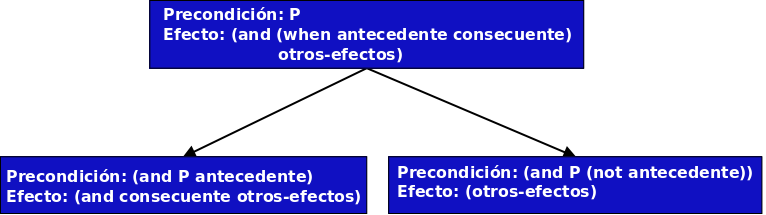
\includegraphics[width=10cm,height=3.5cm]{ef.png}\end{center}

\end{itemize} % ends low level
\end{frame}
\begin{frame}
\frametitle{Anexo (3) - Diagrama de Traducción}
\label{sec-6.11}

\begin{center} 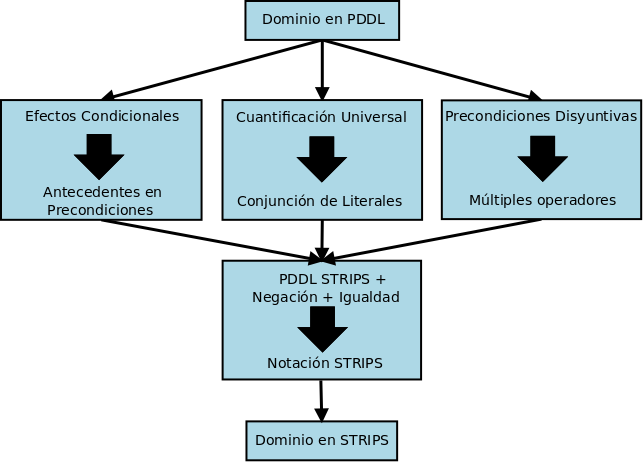
\includegraphics[width=9cm,height=7.5cm]{capastrad.png} \end{center}
\end{frame}

\end{document}
